%----------------------------------------
\begin{frame}
  \frametitle{Part 1}

\icontest[3.2]

\vspace{0.45cm}

{\Large\bf Testing: the execution does not exist yet}

\vspace{0.4cm}

{\small \fuzz{}, built on \matl{} and \zthree{}}

\end{frame}

%----------------------------------------
\begin{frame}
  \frametitle{Fuzzing a command-driven system} \small

\begin{figure}
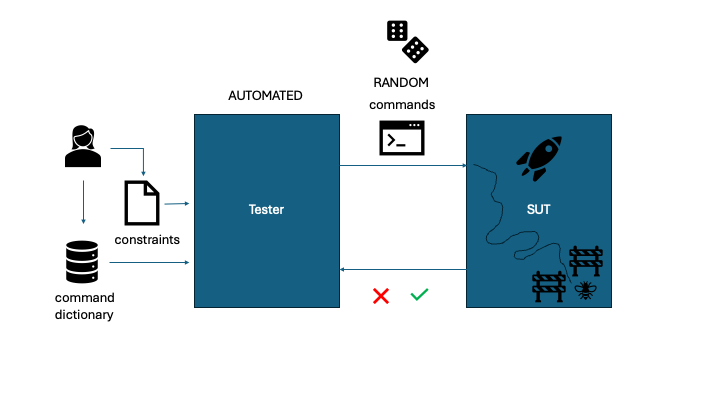
\includegraphics[width=0.62\textwidth]{figures/start5.png}
\end{figure}

Spacecraft are operated by {\bf sequences of commands}, tested by hand-written ones
that do not reach the corners. Random sequences do, but are rejected as illegal.

\pause
\vspace{0.15cm}

\begin{block}{}\small
\centering
So: {\bf constrain the randomness}. The user says what a legal sequence looks
like, in temporal logic; we generate random sequences satisfying it.
\end{block}

\end{frame}

%----------------------------------------
\begin{frame}[fragile]
  \frametitle{From temporal logic to a solver} \small

The specification language is {\bf \matl{}} --- temporal logic over events that
carry data, with binding. {\em Every sample collected is eventually downlinked}:
\[
\Box (\mathit{COLLECT}(file=f?) \Rightarrow \Diamond\, \mathit{SEND}(file=f))
\]

\pause
\vspace{-0.1cm}

A test is a function from position to command, and the formula becomes a constraint
on it. Writing $p$ for the {\tt COLLECT} and $q$ for the matching {\tt SEND},
unfolding over length 3:

\vspace{-0.2cm}

\begin{align*}
&\neg p(test(0)) \vee q(test(0)) \vee q(test(1)) \vee q(test(2)) \\
\wedge\quad &\neg p(test(1)) \vee q(test(1)) \vee q(test(2)) \\
\wedge\quad &\neg p(test(2)) \vee q(test(2))
\end{align*}

\vspace{-0.15cm}

\pause

Hand that to {\bf \zthree{}}, and a satisfying assignment {\em is} a legal test:

\begin{lstlisting}[language=python]
{'name': 'COLLECT', 'number': 1, 'time': 363, 'file': 'img042'}
{'name': 'COLLECT', 'number': 2, 'time': 373, 'file': 'log007'}
{'name': 'SEND',    'number': 3, 'time': 383, 'file': 'img042'}
{'name': 'SEND',    'number': 4, 'time': 394, 'file': 'log007'}
\end{lstlisting}

\vspace{-0.15cm}

Two collections outstanding at once, and {\em both} downlinked --- the binding on
$f$ is what makes that a real obligation rather than one \tool{SEND} satisfying
everything.

\end{frame}
